\documentclass[a4paper,12pt]{article}

\usepackage{graphicx}   % Imágenes
\usepackage{helvet}     % Fuente de letra
\usepackage[hidelinks]{hyperref}   % Tabla de contenido
\usepackage{url}
\usepackage{etoolbox}
\usepackage{setspace}   % Interlineado
\usepackage{geometry}   % Márgenes
\usepackage{tabularx}   % Tablas

% Márgenes
\geometry{
    a4paper,
    left=25mm,
    right=25mm,
    top=25mm,
    bottom=25mm
}

% Eliminar título de la bibliografía
\patchcmd{\thebibliography}{\section*{\refname}}{}{}{}

\onehalfspacing

\renewcommand{\familydefault}{\sfdefault}
\renewcommand{\contentsname}{Tabla de contenidos}

% Configuración de la portada
\begin{document}

\begin{titlepage}
    \centering
    \vspace*{0.5cm}

    % Logo de la universidad
    
\includegraphics[width=1\textwidth]{logo-tec.png}\par\vspace{1cm}

    % Nombre de la universidad
    {\scshape Instituto Tecnológico de Costa Rica\par}
    \vspace{2cm}

    % Título
    {\Huge\bfseries Proyecto \#1: Scanner\par}
    \vspace{2cm}

    % Escuela
    {\large Escuela de Ingeniería en Computación\par}

    % Curso
    {\large Compiladores e Intérpretes IC-5701\par}
    \vspace{2cm}

    % Autor
    {\large Alonso Navarro Carrillo, c. 2022236435\par}
    \vspace{0.25cm}
    {\large Carlos Venegas Masis, c. 2022153870 \par}
    \vspace{0.25cm}
    {\large Valeria, c. \par}
    \vspace{2cm}

    \vfill

    % Profesor
    {\large Ing. Ericka Marín Schumann\par}

    % Semestre
    {II Semestre 2024\par}
\end{titlepage}

\tableofcontents\newpage

% Introducción
\section*{Introducción}
\addcontentsline{toc}{section}{Introducción}
\begin{flushleft}
	\hspace*{2em} Este proyecto se sitúa en la primera etapa del desarrollo
de un compilador para el lenguaje de programación C, conocida como el
Análisis Léxico. El objetivo principal de esta etapa es diseñar y construir
un scanner que sea capaz de identificar y clasificar los diferentes tokens
que conforman un programa en C. Para lograr esto, se utilizó la herramienta
JFlex, la cual permite definir expresiones regulares que describen los patrones
de los tokens a reconocer.
\end{flushleft}

% Estrategia de solución
\section*{Estrategia de solución}
\addcontentsline{toc}{section}{Estrategia de solución}
\begin{flushleft}
    \hspace*{2em} Después de leer detenidamente la documentación 
    de JFlex, se comenzó a diseñar las expresiones regulares 
    para los tokens que debía reconocer el escáner. Aquí surgió 
    el primer problema: el escáner reconoce los tokens según 
    el orden de prioridad. Es decir, si la primera expresión 
    regular es un punto, ningún otro token será reconocido, 
    ya que este metacaracter coincide con cualquier carácter, 
    interpretándolo como un error. Por lo tanto, fue crucial 
    definir adecuadamente el orden de las expresiones regulares. \par
    \vspace{1em}
    \hspace*{2em} Una vez definido el orden de las expresiones 
    regulares, procedimos a diseñar la estructura de los tokens 
    y sus tipos. Para ello, decidimos crear un mapa que facilitara 
    la búsqueda de tokens repetidos en el documento. De manera 
    similar, cada token guarda las líneas en las que aparece 
    en un mapa, lo que permite incrementar el contador de 
    ocurrencias de un token en una misma línea. Finalmente, 
    los tipos de tokens se almacenan en un enum. \par
    \vspace{1em}
    \hspace*{2em} Por último, se implementaron errores 
    definidos, como un número seguido de un identificador 
    o números flotantes que comienzan con un punto. Era 
    necesario definir estos errores como tokens para que 
    pudieran ser reconocidos por el escáner. Los errores no 
    se almacenan en una estructura de datos; en su lugar, se 
    imprimen directamente y no se agregan al mapa de tokens. \par
    \vspace{1em}
\end{flushleft}

\newpage

% Análisis de resultados
\section*{Análisis de resultados}
\addcontentsline{toc}{section}{Análisis de resultados}
\begin{table}[!ht]
    \centering
    \begin{tabularx}{\textwidth}{|X|X|X|}
        \hline
        Actividad & Porcentaje realizado & Justificación \\ 
        \hline
        Desplegar lista de errores léxicos & 100\% & \\
        \hline
        Desplegar listado de tokens encontrados & 100\% & \\
        \hline
        Mostrar tipo de token, línea y cantidad de apariciones por cada token & 100\% & \\
        \hline
        Manejar 4 tipos grandes (operadores, literales, ids, palabras reservadas) de tokens & 100\% & \\
        \hline
        Ignorar comentarios en línea y bloque & 100\% & \\
        \hline
        Identificar todos los operadores válidos de C & 100\% & \\
        \hline
        Identificar todos los literales válidos de C & 100\% & \\
        \hline
        Identificar todos los identificadores válidos de C & 100\% & \\
        \hline
        Identificar todas las palabras reservadas de C & 100\% & \\
        \hline
        Definir errores léxicos & 100\% & \\
        \hline
    \end{tabularx}
\end{table}

% Lecciones aprendidas
\section*{Lecciones aprendidas}
\addcontentsline{toc}{section}{Lecciones aprendidas}

% Casos de prueba
\section*{Casos de prueba}
\addcontentsline{toc}{section}{Casos de prueba}

% Manual de usuario
\section*{Manual de usuario}
\addcontentsline{toc}{section}{Manual de usuario}
\subsection*{Instalación}
Para construir y ejecutar el proyecto, es necesario tener Java instalado en tu sistema. Sigue estos pasos para configurar el proyecto:

\begin{enumerate}
    \item Clona el repositorio:
    \begin{verbatim}
    git clone https://github.com/AlonsoNav/CCompilerJFlex.git
    cd your-repo
    \end{verbatim}

    \item Genera el archivo \texttt{CLexer}:
    \begin{verbatim}
    java -jar lib/jflex-full-1.9.1.jar src/scanner/CLexer.flex
    \end{verbatim}

    \item Compila el proyecto:
    \begin{verbatim}
    javac -d bin -sourcepath src src/app/Main.java 
    src/scanner/CLexer.java .\src\scanner\Token.java 
    .\src\scanner\TokenType.java 
    \end{verbatim}
\end{enumerate}

\subsection*{Uso}
Para ejecutar el compilador con un archivo de entrada, utiliza el siguiente comando:
\begin{verbatim}
    java -cp bin app.Main input_file
\end{verbatim}
También puedes enviar la salida a un archivo .txt con
\begin{verbatim}
    java -cp bin app.Main input_file > output.txt
\end{verbatim}

% Bitácora
\section*{Bitácora}
\addcontentsline{toc}{section}{Bitácora}

\subsection*{Fecha: 26-08-2024}
\begin{flushleft}
    \hspace*{2em} En la primera reunión del equipo de trabajo,
    se acordó que CV se encargará de los expresiones regulares
    de los operadores y del formato de impresión de la tabla.
    AN diseñará la estructura de los tokens y sus errores, 
    así como las expresiones regulares de los identificadores
    y palabras reservadas. VG se responsabilizará de los 
    literales. Por último, se decidió que la documentación se 
    realizará en LaTeX y que GitHub será utilizado como 
    sistema de control de versiones.
\end{flushleft}

\subsection*{Fecha: 01-09-2024}
\begin{flushleft}
    La profesora responde las siguientes consultas:
    \begin{itemize}
        \item Nosotros ya manejamos los diferentes tipos de 
        tokens en un enum. Queremos agregar subtipos pensando 
        a futuro, pero no sé si sea mejor manejar cada 
        subtipo de token como una clase aparte o si todo 
        chorreado en un enum funciona. ¿Usted qué me recomienda?
        \item ¿Qué hacemos con las directivas para el procesador 
        como \texttt{\#include} o \texttt{\#define}?
        \item Los literales de los booleanos son 0 (false) y 
        todo lo contrario es true eso lo tomamos como un 
        literal numérico no importa?
        \item Manejamos también sufijos (U: unsigned, L: long...)?
        \item Los errores es necesario guardarlos en una estructura de datos o solo con imprimirlos basta?
    \end{itemize}
    Lo siguiente son las respuestas de la profesora:\par\vspace{1em}
    \centering
    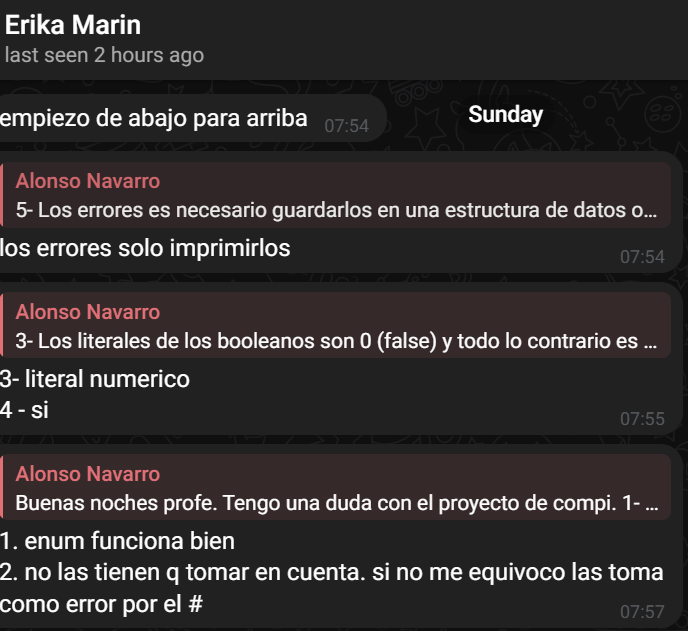
\includegraphics[width=0.5\textwidth]{respuestas-1.png}\par
\end{flushleft}

\subsection*{Fecha: 03-09-2024}
\begin{flushleft}
    La profesora responde la siguiente consulta:
    \begin{quote}
        Usted comentó que cosas como "1ejemplo", debería ser 
        un error y no que los separe como "1": literal y 
        "ejemplo": id. Hay otras cosas que se pegan, por 
        ejemplo con las directivas:
        
        \#include \textless stdio.h \textgreater
        
        lo separa como\par
        \#: error\par
        include: id\par
        \textless operador\par
        stdio: id\par
        . operador\par
        h: id\par
        \textgreater operador\par
        
        Entonces yo ya tengo definido el error genérico de 
        "1ejemplo", pero con esto estaba pensando en meter más 
        caracteres en ese mismo error, pero es que si fuera un 
        "5\textless identificador" en algún condicional ya croma.
    \end{quote}
    La respuesta de la profesora es:\par\vspace{1em}
    \centering
    
\includegraphics[width=0.5\textwidth]{respuestas-2.png}\par
\end{flushleft}

\subsection*{Fecha: 04-09-2024}
\begin{flushleft}
    \hspace*{2em} Luego de tener todo el scanner corriendo 
    correctamente se decide que lo siguiente es finalizar la 
    documentación. CV se encargará de la introducción, AN de 
    la estrategia de solución y VG de las lecciones aprendidas.
    Las demás secciones son redactadas en conjunto. Finalmente,
    se acuerda que cada integrante hará dos casos de prueba y 
    documentará lo encontrado.
\end{flushleft}

% Bibliografía
\newpage
\section*{Bibliografía}
\addcontentsline{toc}{section}{Bibliografía}
\begin{thebibliography}{9}

\bibitem{examplewebsite}
Klein, G., Rowe, S., \& Décamps, R. (marzo de 2023).
\emph{JFlex User’s Manual}.
JFlex Team.
En: \url{https://www.jflex.de/manual.html}.

\end{thebibliography}

\end{document}